\section{Completed matched magnitude-history experiment}

\label{sec:s02-completed}

\textit{Execution provenance: the original completed campaign passed the saved custody checks and predeclared independent raw sample. Acceptance uses sampled validation, not independent replay of every fit. This edition recovered and verified the original histories, selected fit states and attempt records; it did not rerun the fitting campaign.}

The experiment uses 100 paired forest units and 300 catalogues across persistence settings $h\in\{0,0.5,0.9\}$. The strictly subcritical generator has productivity ratio $r=0$ and reproduction mean $n=0.5$. Each catalogue is fitted by M1, the misspecified $r=0.7$ candidate, and M2, the productivity-matched $r=0$ candidate. Both hold $n=0.5$ and use the same inherited kernels and eight-start null/alternative procedure, fitting the background level, trend and stress coefficient. All 600 procedure--catalogue cases are complete; no seed was redrawn.

M1 is a structural replication arm, not an exact numerical replication of the earlier pilot: the common reproduction mean and strengthened starts are disclosed. M2 matches productivity at $h=0$, but the exact Mittag--Leffler generator and finite 195-mode candidate still differ numerically. It is therefore not described as a literally exact full null law.

\begin{table}[htbp]\centering\setlength{\tabcolsep}{5pt}

\caption{Completed selection counts and descriptive empirical calibration. Selection uses $\mathrm{GLR}>0.001$ and $\hat\eta>10^{-6}$. All entries have 100 resolved catalogues; intervals are 95\% Wilson intervals for selection proportions.}\label{tab:s02-completed}

\begin{tabular}{llrrrr}\toprule

Procedure & $h$ & Selected & Wilson interval & Empirical $h=0$ threshold & Above threshold\\\midrule

M1 & 0.0 & 79/100 & [0.700, 0.858] & 7.665955 & 4/100 \\

M1 & 0.5 & 85/100 & [0.767, 0.907] & 7.665955 & 6/100 \\

M1 & 0.9 & 85/100 & [0.767, 0.907] & 7.665955 & 6/100 \\

M2 & 0.0 & 75/100 & [0.657, 0.825] & 4.629883 & 4/100 \\

M2 & 0.5 & 75/100 & [0.657, 0.825] & 4.629883 & 4/100 \\

M2 & 0.9 & 69/100 & [0.594, 0.772] & 4.629883 & 4/100 \\

\bottomrule\end{tabular}\end{table}

The empirical threshold is the higher empirical 95th percentile of the same 100 $h=0$ GLRs within each procedure. The four strict exceedances among those same controls are a consequence of this in-sample construction and ties, not independent evidence of 5\% Type I error control. Selection by the small fixed GLR cutoff and exceedance of this descriptive threshold are distinct summaries.

\begin{table}[htbp]\centering

\caption{Paired GLR changes from $h=0$ on the same forest units. MC SE is a forest-unit sample standard error.}\label{tab:s02-paired}

\begin{tabular}{llrrr}\toprule Procedure & $h$ & Mean change & Median change & MC SE\\\midrule

M1 & 0.5 & -0.009000 & 0.000000 & 0.146627 \\

M1 & 0.9 & 0.010831 & 0.046652 & 0.416236 \\

M2 & 0.5 & -0.106278 & 0.000000 & 0.098682 \\

M2 & 0.9 & -0.140055 & 0.000000 & 0.118097 \\

\bottomrule\end{tabular}\end{table}

\begin{table}[htbp]\centering

\caption{Within-forest M2 minus M1 GLR contrasts. Negative values favour a larger fitted GLR under the misspecified M1 procedure, not better predictive calibration.}

\begin{tabular}{lrr}\toprule $h$ & Mean GLR contrast & MC SE\\\midrule

0.0 & -1.132859 & 0.425666 \\

0.5 & -1.230138 & 0.423813 \\

0.9 & -1.283745 & 0.211306 \\

\bottomrule\end{tabular}\end{table}

These paired results retain all forest units. Neither the large fixed-cutoff selection proportions nor the descriptive self-calibrated thresholds establish a generally valid test for stress inhibition. There is no independent calibration sample in this threshold comparison.

\begin{figure}[htbp]\centering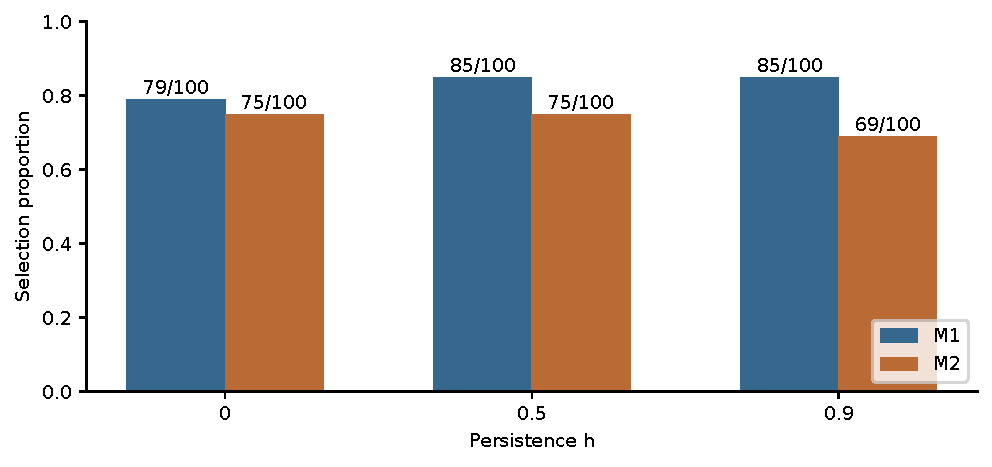
\includegraphics[width=\textwidth]{s02_completed_selection.pdf}\caption{Completed selection proportions under M1 and M2, each based on 100 paired forest units. The display is descriptive; saved custody checks and sampled raw validation passed.}\end{figure}
